\documentclass{article}
\usepackage[style=apa]{biblatex}


\addbibresource{\jobname.bib}
%\AtEveryBibitem{\printfield{note}\clearfield{note}\item}


\usepackage{amsmath}
\usepackage{tikz}
\usetikzlibrary{chains}
\usetikzlibrary{angles, quotes}
\usetikzlibrary{decorations.pathreplacing}
\usepackage{graphicx} % Required for inserting images
\usepackage[T1]{fontenc}
\usepackage{beramono}
\usepackage{courier}
\usepackage{listings}
\usepackage{xpatch}
\usepackage{xcolor}
\usepackage{realboxes}
\usepackage{titlesec}


\setcounter{secnumdepth}{4}


\titleformat{\paragraph}
{\normalfont\normalsize\bfseries}{\theparagraph}{1em}{}
\titlespacing*{\paragraph}
{0pt}{3.25ex plus 1ex minus .2ex}{1.5ex plus .2ex}


\lstdefinelanguage{none}{
  identifierstyle=
}

\definecolor{mygreen}{rgb}{0,0.6,0}
\definecolor{mygray}{rgb}{0.5,0.5,0.5}
\definecolor{mymauve}{rgb}{0.58,0,0.82}
\definecolor{mygray}{rgb}{0.94,0.94,0.94}



%%% Wrap colorbox around lstinline %%%
\makeatletter
\xpretocmd\lstinline{\Colorbox{mygray}\bgroup\appto\lst@DeInit{\egroup}}{}{}
\makeatother
%%%%%%%%%%%%%%%%%%%%%%%%%%%%%%%%%%%%%%

\lstset{ 
  backgroundcolor=\color{mygray},   % choose the background color; you must add \usepackage{color} or \usepackage{xcolor}; should come as last argument
  breakatwhitespace=false,         % sets if automatic breaks should only happen at whitespace
  basicstyle=\ttfamily,
  breaklines=true,                 % sets automatic line breaking
  captionpos=b,                    % sets the caption-position to bottom
  commentstyle=\color{mygreen},    % comment style
  deletekeywords={...},            % if you want to delete keywords from the given language
  escapeinside={\%*}{*)},          % if you want to add LaTeX within your code
  extendedchars=true,              % lets you use non-ASCII characters; for 8-bits encodings only, does not work with UTF-8
  firstnumber=1000,                % start line enumeration with line 1000
  frame=none,	                   % adds a frame around the code
  keepspaces=true,                 % keeps spaces in text, useful for keeping indentation of code (possibly needs columns=flexible)
  keywordstyle=\color{blue},       % keyword style
  language=Octave,                 % the language of the code
  morekeywords={*,...},            % if you want to add more keywords to the set
  numbers=none,                    % where to put the line-numbers; possible values are (none, left, right)
  numbersep=5pt,                   % how far the line-numbers are from the code
  numberstyle=\tiny\color{red}, % the style that is used for the line-numbers
  rulecolor=\color{black},         % if not set, the frame-color may be changed on line-breaks within not-black text (e.g. comments (green here))
  showspaces=false,                % show spaces everywhere adding particular underscores; it overrides 'showstringspaces'
  showstringspaces=false,          % underline spaces within strings only
  showtabs=false,                  % show tabs within strings adding particular underscores
  stepnumber=2,                    % the step between two line-numbers. If it's 1, each line will be numbered
  stringstyle=\color{mymauve},     % string literal style
  tabsize=2,	                   % sets default tabsize to 2 spaces
  title=\lstname                   % show the filename of files included with \lstinputlisting; also try caption instead of title
}

\title{Implementation and comparison of register allocation to translate \lstinline!LLVM--! to x86}
\author{William Welle Tange}
\date{2023}


\begin{document}

\maketitle

\tableofcontents
\newpage

%% TODO: tjek hvad LLVM gør %%


%\texttt{LLVM-{}-2}
%* skab så mange underpunkter som muligt
    %* jo mindre man skal overskue af gangen jo lettere er det at komme i gang med at skrive
    

\section{Introduction}

Compilation refers to the process of translating from one language to another, most often from a high-level programming language intended for humans to work with, to machine- or bytecode intended to be executed on a target platform. This process can be divided into several distinct phases, which are grouped into one of two stages colloquially referred to as the \textit{frontend} and \textit{backend}. The former translating a high-level programming language to an \textit{intermediate representation} (IR) layer and the latter translating IR to executable machine code on a target platform or bytecode for a target \textit{virtual machine} (VM).



\begin{figure}[h]
  \centering
  \resizebox{0.8\textwidth}{!}{
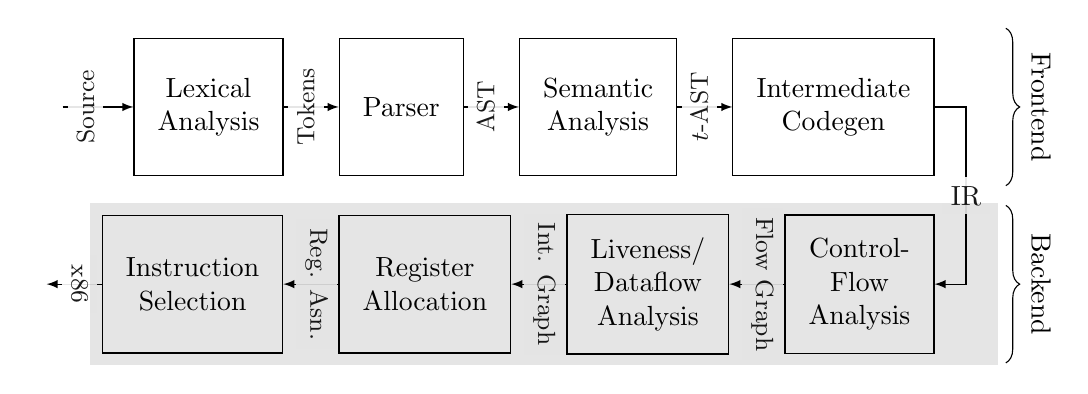
\begin{tikzpicture}
  \tikzset{
box/.style={draw,
  inner sep=0.3cm,
    minimum height=1.75cm,
    align=center},
}


  % Nodes
  \node [box, left, align=center] (incg) at (0,2.25) {Intermediate\\Codegen};
  \node [box, left=0.7 of incg, align=center] (semant) {Semantic\\Analysis};
  \node [box, left=0.7 of semant, align=center] (parse) {Parser};
  \node [box, left=0.7 of parse, align=center] (lex) {Lexical\\Analysis};
  \node [ left=0.9 of lex, align=center] (entry) {};
  \node [box, left, align=center] (cfa) at (0,0) {Control-\\Flow\\Analysis};
  \node [box, left=0.7 of cfa, align=center] (lva)  {Liveness/\\Dataflow\\Analysis};
  \node [box, left=0.7 of lva, align=center] (alloc)  {Register\\Allocation};
  \node [box, left=0.7 of alloc, align=center] (x86)  {Instruction\\Selection};
  \node [ left=0.70 of x86, align=center] (exit) {};

  % Edge with right-angle corners
  \draw [-latex] (entry.east) -- (lex.west)  node [near start,pos=0.325,rotate=90,fill=white,opacity=0.9] {\small Source};
  \draw [-latex] (lex.east) -- (parse.west)  node [midway,pos=0.4,rotate=90,fill=white,opacity=0.9] {\small Tokens};
  \draw [-latex] (parse.east) -- (semant.west)  node [midway,pos=0.4,rotate=90,fill=white,opacity=0.9] {\small AST};
  \draw [-latex] (semant.east) -- (incg.west)  node [midway,pos=0.4,rotate=90,fill=white,opacity=0.9] {\small \(t\)-AST};
  \draw [-latex] (incg.east) -- +(0.4,0) |- node[pos=0.25,fill=white,opacity=0.9] {IR} (cfa.east);
  \draw [-latex] (cfa.west) -- (lva.east)  node [midway,pos=0.4,rotate=-90,fill=white,opacity=0.9] {\small Flow Graph};
  \draw [-latex] (lva.west) -- (alloc.east)  node [midway,pos=0.4,rotate=-90,fill=white,opacity=0.9] {\small Int. Graph};
  \draw [-latex] (alloc.west) -- (x86.east)  node [midway,pos=0.4,rotate=-90,fill=white,opacity=0.9] {\small Reg. Asn.};
  \draw [-latex] (x86.west) -- (exit.east)  node [midway,pos=0.4,rotate=-90,fill=white,opacity=0.9] {\small x86};

  % backend outline
  \fill [opacity=0.1] ([shift={(-0.15,-0.15)}]x86.south west) rectangle ([shift={(0.8,0.15)}]cfa.north east);

  \draw [decorate,decoration={brace,amplitude=5pt,mirror,raise=4ex}]
    (0.3,-1) -- (0.3,1) node[midway,xshift=3em,rotate=-90]{Backend};
  \draw [decorate,decoration={brace,amplitude=5pt,mirror,raise=4ex}]
    (0.3,1.25) -- (0.3,3.25) node[midway,xshift=3em,rotate=-90]{Frontend};
\end{tikzpicture}}
\caption{Compiler phases, backend highlighted}
\end{figure}
Most operations of a general-purpose programming language are translated to a set of logic,  control, and arithmetic instructions that are intended to be executed sequentially on a computer processor: a single circuit/chip, referred to as the \textit{central processing unit} (CPU). CPU design varies and has evolved over time, but most processors executing logic operations are \textit{register machines}, in that they use a limited set of \textit{general-purpose registers} (GPRs) to store working values in combination with \textit{random access memory} (RAM) for mid-term and other I/O peripherals for long-term storage.

This can largely be attributed to performance, as register machines routinely outperform so-called \textit{stack machines} \parencite{ShiYunhe2008VmsS} that are often used in VMs.
Because of the limited amount of GPRs available simultaneously, a crucial part of the backend stage for an optimizing compiler is assigning each variable  of the source program to a GPR in such a way that maximizes performance without sacrificing correctness.

The process of assigning each variable to a GPR is referred to as \textit{register allocation}, and can be approached in several different ways. This paper will seek to implement graph coloring and linear scan and evaluate them in terms of runtime performance after compilation. %% TODO: compare with time-complexity/compile-time duration?
The primary sources will be \textit{Modern Compiler Implementation in ML} \parencite{tiger} and \textit{Compilers: Principles, techniques, and tools} \parencite{dragon}, in addition to publications concerning the linear scan approach.


%* overfladisk intro til hvad helvede register allokering er og hvorfor
    %* hovedtræk
%* rudimentær del af compilation/oversættelse fra high-level sprog til x86 er register allokering
    %* projektet er skridtet videre fra compilers kurset
    %* siger hvad jeg står ovenpå/bygger på
%snak om hvorfor jeg valgte llvm/ssa frem for x86 til global register llocation


\section{Review of Literature}

The two primary sources are the \textit{Modern Compiler Implementation in ML} \cite{tiger} and Dragonbook \cite{dragon}, in addition to scientific publications concerning the linear scan approach.

\subsection{Control Flow Analysis}

The backend of a compiler takes some form of IR as input, usually a linear sequence of instructions for each separate function. This representation is close to the level of an actual processor by design, but it isn't immediately useful for the further analysis steps needed to generate optimized code for the target architecture. %%(FIXME: why not?)
The control flow of a given program refers to the order in which instructions are executed. While the flow of most instructions is linear, in the sense that the next instruction to be executed is located immediately after, some send the execution elsewhere or outright terminate it. %% FIXME: why is this important?

% mention basic block early on, they're a contiguous sequence of instructions that do not transfer control flow

These contiguous sequences of instructions are referred to as \textit{basic blocks}: a basic block is defined as a sequence of instructions with no branches in or out except for the first and last instructions, and can be collectively construed of as a node in a control flow graph, whose directed entry edges are from any block that directs control flow towards itself.

These instructions are referred to as \textit{terminators}, as they potentially terminate a contiguous flow of execution. This subset of instructions can be further divided into \textit{branch instructions} and those concerned with handling the callstack in function/subroutine management.

%These so-called \textit{branch instructions} that alter the flow of execution are further c








hence a \textit{control flow graph} is derived from these. A terminator will branch elsewhere to continue execution. The destination of this has to be an annotated by a label, hence labels \textit{initiate} blocks.

\subsection{Liveness Analysis}

Liveness analysis is the process of finding the program points at which a variable is live. This serves the function of determining which variables are live simultaneously, i.e. in interference/conflict with one another, which cannot be assigned the same physical register without overwriting the value of one another in execution. These can be derived recursively by iteratively applying so-called \textit{dataflow equations} to each node in a \textit{control-flow graph} (CFG) until a stable state/fixed point is reached.

The algorithm described in \textit{Modern Compiler Implementation in ML} \cite{tiger} and \cite{dragon} is based on the following equations for the live-in and live-out variables respectively:
\begin{align}
  in\left[n\right] &= use\left[n\right] \cup (out\left[n\right] - \mathit{def}\left[n\right])\\
  out\left[n\right] &= \bigcup_{s\in \mathit{succ}\left[n\right]} in\left[s\right]
\end{align}
where \(use\left[n\right]\) is the set of all dependent variables, \(def\left[n\right]\) is the set of all variables defines and \(succ\left[n\right]\) is the set of all immediate successor nodes of \(n\).

The structure of the CFG is inherently vague as both   \cite{tiger} and \textit{Compilers : Principles, Techniques, and Tools} \cite{dragon}, while based on the same underlying % TODO: fix references
conceptions of dataflow, have different approaches to nodes of a CFG, with the former taking each individual instruction into consideration and the latter each basic block. Either of these approaches are sound 


% TODO: try int set instead of symbols

\subsection{Graph Coloring}

\subsection{Linear Scan}

%Write about Appel book.

%Write about SSA form liveness analysis. 

%Keywords: program points, dataflow equations, fixed point




%* todo: ssa/llvm vs appel analysis
%* henvis til blog posts som archive
%    * så tæller det som litteratur
%* tag essensen ud af hvad der bliver sagt i teksten
    %* som er relevant for mit arbejde
%
%* HENVIS TIL KAPITEL 19 OM SSA FORM
%
%* linear scan approach
%
%* snak om hvilke dele af bogen i hvilken rækkefølge
%
%Appel (208p):
%*   Translation To Intermediate Code (153-179, 26p)
%*   Basic Blocks And Traces (179-193, 14p)
%*   Instruction Selection (193-219, 26p)
%*   Liveness Analysis (219-237, 18p)
%*   Register Allocation (237-267, 30p)
%*   Dataflow Analysis (387-415, 28p)
%*   Loop Optimizations (415-439, 24p)
%*   Static Single Assignment Form (439-481, 42p)
%
%*using IR when only translating from one language to another:
%
%>Even when only one front end and one back end are being built, a good IR can modularize the task, so that the front end is not complicated with machine-specific details, and the back end is not bothered with information specific to one source language.

\section{\lstinline!LLVM--! instruction set}

The intermediate representation emitted by the frontend of a compiler serves as a stepping stone independent of the target architecture. The \lstinline!LLVM! infrastructure is the industry standard in terms of bridging this gap and was consequently the library used to translate the semantically annotated abstract syntax tree to executable machine code in the 2022 compilers course. As this project is an expansion on this, it follows naturally to build on this. 

The instruction set used in this paper will be a union of the sets used in the 2022 and 2023 compilers courses in order to work as a drop-in replacement of LLVM for either of the two respective source languages:  Tiger and Dolphin. This instruction set is a subset of the one used in practice, as, for instance, neither of the languages implemented support exception handling, floating point operations and so on, and instead only strive to cover the basics of compilers.

The instructions included are
\lstinline!trunc! has only been added in order to help cover more generated LLVM.
%with only four distinct block terminators 
%\begin{enumerate}
%    \item Unconditional \lstinline!br! followed by the label to branch to
%    \item Conditional \lstinline!br!  followed by an \lstinline!i1! condition and two labels
%    \item \lstinline!ret! followed by an optional return value
%    \item \lstinline!unreachable!
%\end{enumerate}
The branching for most of these is trivial: after successful execution the flow of all but \lstinline!br!, \lstinline!ret! and \lstinline!unreachable! will unconditionally attempt to execute the next instruction in memory (i.e. increment the instruction pointer by instruction length).

Because of this, these instructions are referred to as \textit{terminators}, as their purpose is to disrupt what had otherwise been a linear flow from the beginning of this continus sequence of instructions, henceforth referred to as a \textit{basic block}.

\section{Control Flow Analysis}


With an input stream of instructions 

%* description of blocks, how they connect etc.

Each function defined in an LLVM program is constructed with the help of

\section{Liveness Analysis}

Dataflow analysis 


%\section{CFG -> INTERF}

%* describe the dataflow algorithm from the book
%* describe the interference criteria from the book

%\section{INTERF -> DOT}

%* ez ???

%\section{INTERF -> DOT/Assignment}

%* list of methods for coalescing/allocating:
%   * ocamlgraph builtin
%   * greedy 
%   * briggs
%   * george
%   * welsh-powell?
\section{Graph Coloring}
The graph coloring by simplification as described by Appel 

%% TODO
%* optimistic coloring
\subsection{Coalescing}


\section{Linear Scan}

%Live ranges for each of the temporaries are derived by visiting each instruction of each control flow block and examining its \textit{uses} and \textit{defs}.

\section{Instruction Selection}

Translating each IR instruction to x86 correctly is a matter of eliminating unintended side-effects. Each LLVM-- instruction is defined to have only one purpose, %% FIXME is purpose the right word?
as concepts such as calling conventions, stack frames, or a \lstinline!FLAGS! register are completely abstracted over in order to remain platform independent.

In contrast, the x86 \textit{instruction set architecture} (ISA) is targeting a  \textit{complex instruction set computer} (CISC) family of processors, the instructions of which perform a much broader set of operations \cite[p.~190]{tiger}. This is is in part due to pipelining, i.e. an abstraction over the concrete implementation of the actual processor, which in turn is made for the sake of performance.

An example of this would be the division/remainder operation: since integer division is a non-trivial iterative process wherein both the quotient and remainder is needed throughout, the result of both of these is stored in the \lstinline!%rax! and \lstinline!%rdx! registers respectively. This means two operations are performed simultaneously regardless of which value is used, hence they need to be restored before executing the next instruction, as any variables assigned to \lstinline!%rax! or \lstinline!%rdx! will be overwritten.

\begin{center}
\begin{tabular}{|c||c|c|c|c|} 
 \hline
 add & addx & \{\}\\
 \hline
 mul & imul & \{ \%rax \} \\
 \hline
 sdiv & idivx & \{\%rax, \%rdx\} \\
 \hline
 srem & idivx & \{\%rax, \%rdx \\
 \hline
   call & callx & \{\%rax, \textit{caller saved registers}\} \\
 \hline
 \hline
\end{tabular}
\end{center}

%* safest possible x86 translation
%
    %* moving sys-v abi arguments to assigned registers is treacherous

\section{Further Optimization}

% TODO: quote computability theory infinitely many optimizations


\section{Evaluation}

Relevant metrics by which to compare these variations are naturally the performance of the code generated at runtime, but also the time efficiency at compile-time. While the code written isn't expected to outperform LLVM, due to the time complexity of the linear scan and simplification algorithms implemented their respective runtime performances are expected to outperform the builtin graph coloring algorithm.

% TODO: cpu cycles

Another factor worth considering would be memory usage, caches misses, garbage collection (although not relevant to this as it doesn't use GC), vectorizatiion (loop optimizations by SIMD) etc.

\subsection{Benchmarking}

Benchmarks are performed on Apple Silicon (M1 Pro, i.e. ARMv8.5-A \cite{article}) despite the target instruction set being x86-64. This is possible because of Rosetta 2, which  translates x86-64 to ARMv8 before execution \cite{PolettoMassimiliano1999Lsra}.  Time is measured using the \lstinline!time! function of the bash shell as it is native to the chosen Docker image.  As all execution relevant to the performance of register allocation is done in user mode, only the \lstinline!user! metric is noted.

%* fib
%* ack
%* \lstinline!/usr/bin/time -al! counts cpu cycles

%Benchmarks are performed in the environment described by the Dockerfile in the repository and executed on an Apple Silicon/M1 chip. Time is measured using the \lstinline!time! function of the bash shell as it is native to the chosen Docker image.  As all execution relevant to the performance of register allocation is done in user mode, only the \lstinline!user! metric is noted.

%TODO:
%
%* should I use shell time, or /usr/bin/time?
%* how do I measure cpu cycles?
\begin{center}
\begin{tabular}{ c c c }
 cell1 & cell2 & cell3 \\ 
 cell4 & cell5 & cell6 \\  
 cell7 & cell8 & cell9    
\end{tabular}
\end{center}

\begin{center}
\begin{tabular}{|c||c|c|c|c|} 
 \hline
 fib & clang & greedy & briggs & linear \\ [0.5ex] 
 \hline
 40 & 1.000000 & 1.438693 & 1.441270 & 0.73 \\ [1ex] 
 41 & 1.000000 & 1.441035 & 1.440626 & 0.73 \\ [1ex] 
 \hline
\end{tabular}
\end{center}

 


bench clang	benches/fib.ll 42 	min=5494929992 (1.000000)	avg=5545852373 (1.000000)	max=5669289413
bench greedy	benches/fib.ll 42 	min=7951933724 (1.447140)	avg=7969947833 (1.437101)	max=8004638438
bench briggs	benches/fib.ll 42 	min=7946186345 (1.446094)

\begin{center}
\begin{tabular}{|c||c|c|c|c|} 
 \hline
 sha256 & clang & greedy & briggs & linear \\ [0.5ex] 
 \hline
 1000000 & 1 & 0.73 & 0.73 & 0.73 \\ [1ex] 
 \hline
\end{tabular}
\end{center}


\subsection{Comparison to other work and ideas for future work}


\section{Conclusion}



%\defbibnote{myprenote}{This thesis is based on the following original publications:}
%\printbibliography[prenote=myprenote,title={References}]
%\printbibliography[title={References}]

\printbibliography 


\appendix

\newpage

%%% NOTE: Don't include subsections of tthe benchmarks section
\addtocontents{toc}{\protect\setcounter{tocdepth}{1}}

\section{LLVM-- instruction set}
\label{appendix:llvmis}
\begin{enumerate}
    \item binary operations \lstinline!add!, \lstinline!and!, \lstinline!ashr!, \lstinline!lshr!, \lstinline!mul!, \lstinline!or!, \lstinline!sdiv!,\\\lstinline!srem!, \lstinline!shl!, \lstinline!sub! and \lstinline!xor!
    \item integer comparison \lstinline!icmp! (conditions being \lstinline!eq!, \lstinline!ne!, \lstinline!sge!, \lstinline!sgt!, \lstinline!sle! and \lstinline!slt!)
    \item memory/address operations \lstinline!alloca!, \lstinline!gep!, \lstinline!load! and \lstinline!store!
    \item  \lstinline!mov! operations \lstinline!gep!, \lstinline!phi!, \lstinline!ptrtoint!, \lstinline!trunc!, and \lstinline!zext!
    \item control flow operations \lstinline!br!, \lstinline!call! and \lstinline!ret!
    \item a  nullary block terminator \lstinline!unreachable!
\end{enumerate}

\section{Benchmarks}

\subsection{\lstinline!benches/fib.ll!}
\begin{lstlisting}[language=LLVM]
declare i32 @atoi(i8*)
define i32 @fib(i32 %n0) {
  %cn =  icmp sle i32 %n0, 2
  br i1 %cn, label %base, label %rec
base:
  ret i32 1
rec:
  %n1 = sub i32 %n0, 1
  %v0 = call i32 @fib(i32 %n1)
  %n2 = sub i32 %n0, 2
  %v1 = call i32 @fib(i32 %n2)
  %v2 = add i32 %v1, %v2
  ret i32 %v2
}
define i32 @main(i32 %argc, i8** %argv) {
  %arg1ptr = getelementptr i8*, i8** %argv, i64 1
  %arg1 = load i8*, i8** %arg1ptr
  %n = call i32 @atoi(i8* %arg1)
  call i32 @fib(i32 %n)
  ret i32 0
}

\end{lstlisting}

\subsubsection{\lstinline!make fib-clang!}
\begin{lstlisting}[language=none]
$ make fib-clang
clang -O0 -target x86_64-unknown-darwin benches/fib.ll -o fib-clang
\end{lstlisting}
\paragraph{\lstinline!make bench fib-clang 42!}
\begin{lstlisting}[language=none]
$ make bench fib-clang 42
/usr/bin/time -al ./fib-clang 42
        1.58 real         1.56 user         0.00 sys
             2678784  maximum resident set size
                   0  average shared memory size
                   0  average unshared data size
                   0  average unshared stack size
                 765  page reclaims
                   0  page faults
                   0  swaps
                   0  block input operations
                   0  block output operations
                   0  messages sent
                   0  messages received
                   0  signals received
                   0  voluntary context switches
                  29  involuntary context switches
         11000239251  instructions retired
          4962802652  cycles elapsed
             1708928  peak memory footprint
\end{lstlisting}
\paragraph{\lstinline!make bench fib-clang 43!}
\begin{lstlisting}[language=none]
make bench fib-clang 43
$ /usr/bin/time -al ./fib-clang 43
        2.71 real         2.49 user         0.00 sys
             2678784  maximum resident set size
                   0  average shared memory size
                   0  average unshared data size
                   0  average unshared stack size
                 700  page reclaims
                  66  page faults
                   0  swaps
                   0  block input operations
                   0  block output operations
                   0  messages sent
                   0  messages received
                   0  signals received
                  13  voluntary context switches
                  32  involuntary context switches
         17797124508  instructions retired
          8035601598  cycles elapsed
             1708928  peak memory footprint
\end{lstlisting}

\paragraph{\lstinline!make bench fib-clang 44!}
\begin{lstlisting}[language=none]
$ make bench fib-clang 44
/usr/bin/time -al ./fib-clang 44
        4.06 real         4.04 user         0.00 sys
             2678784  maximum resident set size
                   0  average shared memory size
                   0  average unshared data size
                   0  average unshared stack size
                 700  page reclaims
                  66  page faults
                   0  swaps
                   0  block input operations
                   0  block output operations
                   0  messages sent
                   0  messages received
                   0  signals received
                   5  voluntary context switches
                  29  involuntary context switches
         28781328564  instructions retired
         12988681489  cycles elapsed
             1708928  peak memory footprint
\end{lstlisting}


\paragraph{\lstinline!make bench fib-clang 45!}
\begin{lstlisting}[language=none]
$ make bench fib-clang 45
/usr/bin/time -al ./fib-clang 45
        6.54 real         6.51 user         0.00 sys
             2678784  maximum resident set size
                   0  average shared memory size
                   0  average unshared data size
                   0  average unshared stack size
                 700  page reclaims
                  66  page faults
                   0  swaps
                   0  block input operations
                   0  block output operations
                   0  messages sent
                   0  messages received
                   0  signals received
                   6  voluntary context switches
                  39  involuntary context switches
         46555259189  instructions retired
         20968319385  cycles elapsed
             1708928  peak memory footprint
\end{lstlisting}



\paragraph{\lstinline!make bench fib-clang 46!}
\begin{lstlisting}[language=none]
$ make bench fib-clang 46
/usr/bin/time -al ./fib-clang 46
       10.58 real        10.54 user         0.00 sys
             2678784  maximum resident set size
                   0  average shared memory size
                   0  average unshared data size
                   0  average unshared stack size
                 700  page reclaims
                  66  page faults
                   0  swaps
                   0  block input operations
                   0  block output operations
                   0  messages sent
                   0  messages received
                   0  signals received
                   5  voluntary context switches
                 107  involuntary context switches
         75314385847  instructions retired
         33939361073  cycles elapsed
             1725376  peak memory footprint
\end{lstlisting}



\paragraph{\lstinline!make bench fib-clang 47!}
\begin{lstlisting}[language=none]
$ make bench fib-clang 47
/usr/bin/time -al ./fib-clang 47
       17.09 real        17.06 user         0.00 sys
             2678784  maximum resident set size
                   0  average shared memory size
                   0  average unshared data size
                   0  average unshared stack size
                 766  page reclaims
                   0  page faults
                   0  swaps
                   0  block input operations
                   0  block output operations
                   0  messages sent
                   0  messages received
                   0  signals received
                   0  voluntary context switches
                 100  involuntary context switches
        121838577947  instructions retired
         54901966523  cycles elapsed
             1708928  peak memory footprint
\end{lstlisting}



\paragraph{\lstinline!make bench fib-clang 48!}
\begin{lstlisting}[language=none]
$ make bench fib-clang 48
/usr/bin/time -al ./fib-clang 48
       27.65 real        27.59 user         0.00 sys
             2678784  maximum resident set size
                   0  average shared memory size
                   0  average unshared data size
                   0  average unshared stack size
                 766  page reclaims
                   0  page faults
                   0  swaps
                   0  block input operations
                   0  block output operations
                   0  messages sent
                   0  messages received
                   0  signals received
                   0  voluntary context switches
                 161  involuntary context switches
        197130073055  instructions retired
         88835375488  cycles elapsed
             1708928  peak memory footprint
\end{lstlisting}


\end{document}
